\documentclass[a4paper, 14pt]{article}

\usepackage[english, russian]{babel}
\usepackage[T2A]{fontenc}
\usepackage[utf8]{inputenc}
\usepackage{indentfirst}





\frenchspacing   
\usepackage{amsmath,amsfonts,amssymb,amsthm,mathtools} % пакеты AMS
\usepackage[hidelinks]{hyperref}

\usepackage{icomma}                                    % "Умная" запятая
\usepackage{NiceMatrix}

\usepackage{physics}

\usepackage{tikz}
\usepackage{geometry}
\geometry{top=25mm}
\geometry{bottom=30mm}
\geometry{left=20mm}
\geometry{right=20mm}

\linespread{1}

%Колонтитулы
\usepackage{titleps}
\newpagestyle{main}{
	\setheadrule{0.4pt}
	\setfootrule{0.4pt}
	\setfoot{}{\thepage}{}
}
\pagestyle{main}
\newcommand{\deriv}[2]{\frac{\partial #1}{\partial #2}}
\newcommand{\cderiv}[2]{\cfrac{\partial #1}{\partial #2}}
\newcommand*{\Eval}[3]{\left.#1\right\rvert_{#2}^{#3}}

\usepackage{color}
\usepackage{listings}

\lstdefinestyle{customc}{
	belowcaptionskip=1\baselineskip,
	breaklines=true,
	frame=L,
	xleftmargin=\parindent,
	language=C++,
	showstringspaces=false,
	basicstyle=\footnotesize\ttfamily,
	keywordstyle=\bfseries\color{green!40!black},
	commentstyle=\itshape\color{purple!40!black},
	identifierstyle=\color{blue},
	stringstyle=\color{orange},
}

\lstdefinestyle{customasm}{
	belowcaptionskip=1\baselineskip,
	frame=L,
	xleftmargin=\parindent,
	language=[x86masm]Assembler,
	basicstyle=\footnotesize\ttfamily,
	commentstyle=\itshape\color{purple!40!black},
}

\lstset{escapechar=@,style=customc}


\begin{document}
	\section{Генерация}
	Для интегрирования методом МК нужно соответствующие дифференциалы заменить на веса и функции от генераторов.
	
	Положим $G()$ --- генератор случайнгого числа от $0..1$ не включительно.
	
	Полная скорость захвата это интеграл
	\begin{equation*}
		\label{eq:capture_rate}
		C_{+} = {\int{d^{3}\vec{r} \cdot d^{3}\vec{v}f_{k}\left( {r,v} \right) \cdot n_{p}f_{B}\left( {\vec{v}}_{1} \right)d^{3}{\vec{v}}_{1} \cdot \Gamma_{с}\left( \vec{v},{\vec{v}}_{1},r \right)}}
	\end{equation*}
	где
	\begin{equation*}
		\label{eq:Gamma_def}
		\Gamma_{с}\left( {\vec{v},{\vec{v}}_{1},r} \right) = {\int\limits_{v' < v_{esc}}{d^{3}{\vec{v}}\,'\delta\left( {E_{f} - E_{in}} \right) \cdot \frac{m_{k}^{3}\left| \mathcal{M} \right|^{2}}{64\pi^{2}m_{i}^{2}m_{k}^{2}}}} = 
		\int{ |\vec{v}-\vec{v}_1|d\sigma }
	\end{equation*}
	--- сечение, умноженное на разность скоростей.
	\begin{equation*}
		\Gamma_{с}\left( {\vec{v},{\vec{v}}_{1},r} \right) = \nu' d\vec{n}\,'\frac{G_{F}^{2}}{\pi}\frac{m_i m_{k}^{2}}{\left( m_{i} + m_{k} \right)}\Phi dF
	\end{equation*}
	\begin{itemize}
		\item Генерация $d^3\vec{r}$
		\begin{equation*}
			d^3\vec{r} = V\cdot 3 \xi^2 d\xi
		\end{equation*}
		где $\xi$ --- безразмерный радиус
		
		Положим $\xi = G()^{n} = g_1^n$
		\begin{equation*}
			d^3\vec{r} = V\cdot 3n g_1^{3n-1} d g_1 = V3n\xi^{\frac{3n-1}{p}} d g_1
		\end{equation*}
		
		\begin{lstlisting}
			double r_nd = pow(G(),pow_r);
			factor *= (3*pow_r* pow(r_nd,(3*pow_r-1.0)/pow_r));
		\end{lstlisting}
		
		\item Генерация $d^{3}\vec{v}f_{k}\left( {\vec{r},\vec{v}} \right)$
		
		\begin{equation*}
			d^{3}\vec{v} = 2\pi v dv^2 d\vec{n} = 2\pi v du^2 d\vec{n} = 4\pi vu du d\vec{n}
		\end{equation*}
		\begin{equation*}
			f_{k}\left( {\vec{r},\vec{v}} \right) = n_{\chi}f(u) 
		\end{equation*}
		\begin{equation*}
			f(u) = \cfrac{1}{2 (2\pi)^{3/2}u v_{\odot} 	\overline{v}} \left(
			e^{-\cfrac{(u-v_{\odot})^2}{2	\overline{v}^2}} - 
			e^{-\cfrac{(u+v_{\odot})^2}{2	\overline{v}^2}}
			\right)
		\end{equation*}
		\begin{equation*}
			v^2 = u^2 + v_{esc}^2
		\end{equation*}
		За генерацию скорости отвечает функция Velocity(). Причем напрвление скоростей считается изотропным. Под $d\vec{n}$ подразумевается генерация направления.
		
		Проверка генератора с правильным распределением при $v_{\odot}=0.73e-3, \overline{v} = 0.53e-3,  v_{esc} = 2e-3$
		\begin{figure}[ht]
			\centering
			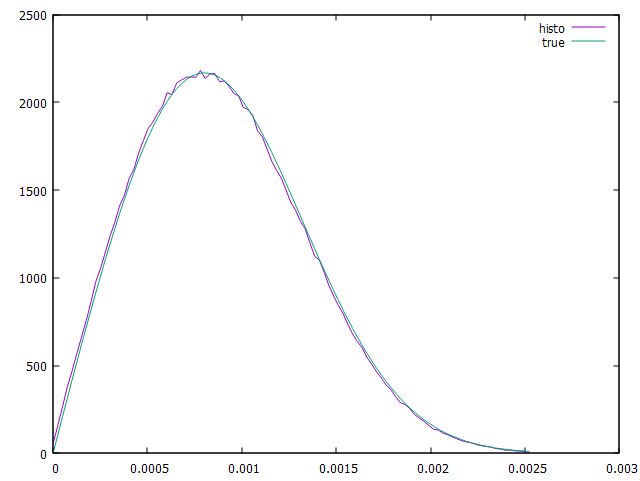
\includegraphics[scale=0.4]{velocity_generator.png}
			\caption{compare of $u$ distribution}
		\end{figure}
		
		\item $f_{B}\left( {\vec{v}}_{1} \right)$:
		\begin{equation*}
			\vec{v}_{1} = Gauss3\left(\sqrt{\frac{T(\xi)}{m_i}}\right)
		\end{equation*}
	
		\item Концентрация ядер $n_i$: $\widehat{\rho}(r) \cdot \widetilde{\rho}_i(r)$ учитывется в коде:
		
		\begin{lstlisting}
			auto /*std::vector<double>*/ RhoND = BM["Rho"];
			...
			decltype(Therm) /*grid function*/ Element_N(R,RhoND*BM[element]);
			...
			double n_nd = nR(r_nd);
			factor *=  n_nd;
		\end{lstlisting}
		\item Массовые константы: из формулы безразмерного захвата осталось только $\frac{m_k}{m_k+m_i}$
		\begin{lstlisting}
			double const_fact_rd = mk/(mk+mi)/Nmk;
		\end{lstlisting}
		
		\item Выходная скорость соответствует интегралу $\nu' d\vec{n}$, где 
		$d\vec{n} = \frac{1}{4\pi} dcos(\theta')d\phi$. С разницей лишь в том, что $cos(\theta')$ генерируется до $cos(\theta_{max})$
		\begin{lstlisting}
			double Nu1_squared =Nu.quad()-deltaE*2*mi/(mk*(mi+mk));
			if(Nu1_squared<=0.0)
			return MC::MCResult<vec3>(vec3(0,0,0),0);
			
			double Nu1 = sqrt(Nu1_squared);
			
			double cosTh1max = (Vesc*Vesc-Nu1_squared-VcmN*VcmN)/(2*VcmN*Nu1);
			...
			double cosTh1 = (1+cosTh1max)*G()-1;
			...
			vec3 vNu1 = Nu1*(n_v*cosTh1+n_1*sinTh1*cos(phi1)+n_2*sinTh1*sin(phi1));
			...
			return MC::MCResult<vec3>(vNu1,0.5*(1.0+cosTh1max)*Nu1);
		\end{lstlisting}
		Из закона сохранения импульса и энергии, выходная скорость частиы в СЦМ изменится
		\begin{equation*}
			\nu'^2 = \nu^2 - \Delta E \cdot \cfrac{2m_i}{m_k(m_i+m_k)}
		\end{equation*}
		
		\item Форм фактор ядра учитывается в структуре dF.
		\begin{lstlisting}
			constexpr double fermi_GeV = 5;
			inline double BesselX(double x) noexcept{
				if(x<0.01){
					return 1.0/3-x*x*(1-x*x/28)/10;
				}else{
					return (sin(x)-x*cos(x))/(x*x*x);
				}
			}
			...
			s =  fermi_GeV*0.9;
			double b = (1.23*pow(M,1.0/3)-0.6)*fermi_GeV;
			double a = 0.52*fermi_GeV;
			R = sqrt(b*b+7*M_PI*M_PI*a*a/3-5*s*s);
			...
			double bf = 3*BesselX(q*R)*exp(-q*q*s*s/2);
			return bf*bf;
		\end{lstlisting}
		
	
	\end{itemize}
\end{document}